% ----------------------------------------------------------
\chapter{FUNDAMENTAÇÃO TEÓRICA} \label{cap:Fundamentacao}
% ----------------------------------------------------------
A arquitetura de software é um dos pilares centrais no desenvolvimento de sistemas computacionais modernos. Ela define a estrutura organizacional de um sistema, estabelecendo diretrizes para a disposição dos seus componentes, suas interações e restrições, além de orientar decisões técnicas que impactam diretamente na escalabilidade, manutenção e evolução do software ao longo do tempo \cite{jamshidi2016systematic}.

De acordo com \cite{jamshidi2016systematic}, a arquitetura de software pode ser compreendida como o conjunto de estruturas necessárias para raciocinar sobre o sistema, que compreende elementos de software, as relações entre eles e as propriedades de ambos. Em outras palavras, a arquitetura de software não se limita apenas à divisão do sistema em módulos, mas também envolve a definição de padrões de comunicação, protocolos, mecanismos de segurança, estratégias de escalabilidade e diretrizes para integração entre componentes. 

A definição de uma arquitetura adequada é fundamental para garantir que o sistema atenda aos requisitos funcionais e não funcionais, como desempenho, segurança, confiabilidade e facilidade de manutenção. Segundo \cite{nizami2020comparison}, a escolha da arquitetura influencia diretamente a capacidade do sistema de evoluir e se adaptar a novas demandas, sendo um fator determinante para o sucesso de projetos de software em ambientes dinâmicos e competitivos.

Historicamente, a arquitetura monolítica foi o modelo predominante no desenvolvimento de sistemas. Nesse paradigma, todas as funcionalidades do software são implementadas em um único bloco, compartilhando o mesmo ambiente de execução, banco de dados e ciclo de vida \cite{nizami2020comparison}. Essa abordagem, embora simples de implementar e gerenciar em projetos de menor escala, apresenta limitações significativas à medida que o sistema cresce, como dificuldades de manutenção, escalabilidade restrita e maior risco de falhas generalizadas. 

Com o avanço das demandas por sistemas mais flexíveis, escaláveis e resilientes, especialmente em ambientes de computação em nuvem, emergiu a arquitetura de microsserviços como uma alternativa ao modelo monolítico \cite{jamshidi2016systematic, shekhar2023microservices}. Os microsserviços propõem a fragmentação do sistema em serviços independentes, cada um responsável por uma funcionalidade específica e comunicando-se por meio de interfaces bem definidas. Essa abordagem permite que equipes distintas desenvolvam, testem e implantem serviços de forma autônoma, promovendo ciclos de entrega mais curtos e maior adaptabilidade às mudanças. 

Além disso, a arquitetura de microsserviços facilita a adoção de práticas modernas de \textit{DevOps}, automação de \textit{deploys} e escalabilidade granular, alinhando-se às necessidades de negócios que exigem respostas rápidas e contínuas às mudanças do mercado \cite{shekhar2023microservices}. No entanto, essa evolução também traz novos desafios, como a necessidade de ferramentas avançadas para orquestração, monitoramento e observabilidade, além de uma curva de aprendizado mais acentuada para as equipes de desenvolvimento \cite{jamshidi2016systematic}. 

A definição de padrões arquiteturais é essencial para garantir a organização, escalabilidade e manutenção de sistemas de software. Diversos padrões foram consolidados na literatura internacional, cada um com características, vantagens e limitações específicas \cite{jamshidi2016systematic}. 

Um dos padrões mais tradicionais é a arquitetura monolítica, na qual todas as funcionalidades do sistema são implementadas em um único bloco de código, compartilhando o mesmo ambiente de execução e banco de dados. Embora seja simples de desenvolver e implantar, esse modelo apresenta dificuldades de escalabilidade e manutenção à medida que o sistema cresce. Como afirmam \cite{nizami2020comparison}: 

“A arquitetura monolítica é fácil de desenvolver e fazer \textit{deploy}, mas, à medida que a aplicação cresce, torna-se difícil de gerenciar, escalar e manter. Qualquer pequena mudança requer que toda a aplicação seja reconstruída e reimplantada, o que aumenta o risco e o esforço.” 

Essa limitação faz com que, em projetos de maior porte, a arquitetura monolítica se torne menos atrativa, especialmente quando há necessidade de frequentes atualizações e escalabilidade do sistema. 

A arquitetura em camadas é amplamente utilizada em sistemas corporativos. Nesse modelo, o sistema é dividido em diferentes camadas, como apresentação, lógica de negócio e acesso a dados, cada uma com responsabilidades bem definidas. Essa separação facilita a manutenção, a reutilização de componentes e a evolução do sistema, além de permitir que equipes distintas trabalhem de forma mais organizada \cite{jamshidi2016systematic}. 

A \textit{Service-Oriented Architecture} (\textit{SOA}) propõe a construção de sistemas a partir de serviços independentes, que se comunicam por meio de protocolos padronizados, como \textit{REST} ou \textit{SOAP}. O \textit{SOA} foi fundamental para a integração de sistemas heterogêneos e para a criação de soluções mais flexíveis, permitindo que diferentes aplicações compartilhem funcionalidades de forma segura e controlada. No entanto, a complexidade de orquestração e a dependência de barramentos de serviço podem tornar a implementação desse padrão mais desafiadora \cite{jamshidi2016systematic}. 

Nos últimos anos, a arquitetura de microsserviços ganhou destaque, principalmente devido à sua capacidade de promover a independência entre equipes, a escalabilidade granular e a facilidade de adoção de práticas modernas de \textit{DevOps}. Cada microsserviço é responsável por uma funcionalidade específica e pode ser desenvolvido, testado, implantado e escalado de forma autônoma. Essa flexibilidade, no entanto, exige um investimento maior em ferramentas de monitoramento, orquestração e observabilidade, além de demandar uma curva de aprendizado mais acentuada para as equipes de desenvolvimento \cite{jamshidi2016systematic, shekhar2023microservices, nizami2020comparison}. 

\section{Padrões Arquiteturais}

\subsection{Arquitetura Monolítica}

A arquitetura monolítica caracteriza-se pela integração de todos os componentes funcionais do sistema - interface de usuário, lógica de negócio e acesso a dados - em uma única unidade de \textit{deploy} e execução \cite{nizami2020comparison}. Nesse modelo, o acoplamento entre módulos é extremamente elevado, uma vez que compartilham o mesmo espaço de memória, base de dados e ciclo de vida. Conforme destacado por \cite{farhan2023performance}, essa estrutura promove rapidez no desenvolvimento inicial devido à simplicidade de configuração e depuração, sendo ideal para protótipos ou sistemas com escopo limitado.

Entretanto, conforme o sistema expande sua base de código e adquire complexidade, emergem desafios significativos:

Escalabilidade vertical obrigatória: A única estratégia viável é a replicação da aplicação inteira, mesmo quando apenas componentes específicos demandam mais recursos \cite{nizami2020comparison}.

Rigidez tecnológica: A adoção de novas tecnologias ou versões requer a atualização do monolito inteiro, gerando \textit{lock-in} e limitando inovação \cite{jamshidi2016systematic}.

Comprometimento da confiabilidade: Falhas em módulos secundários podem paralisar todo o sistema, como demonstrado em testes de carga por \cite{farhan2023performance}.

Complexidade evolutiva: Modificações exigem reteste e reimplantação completos, ampliando riscos e \textit{lead time} para novas funcionalidades.

\begin{figure}[h]
\centering
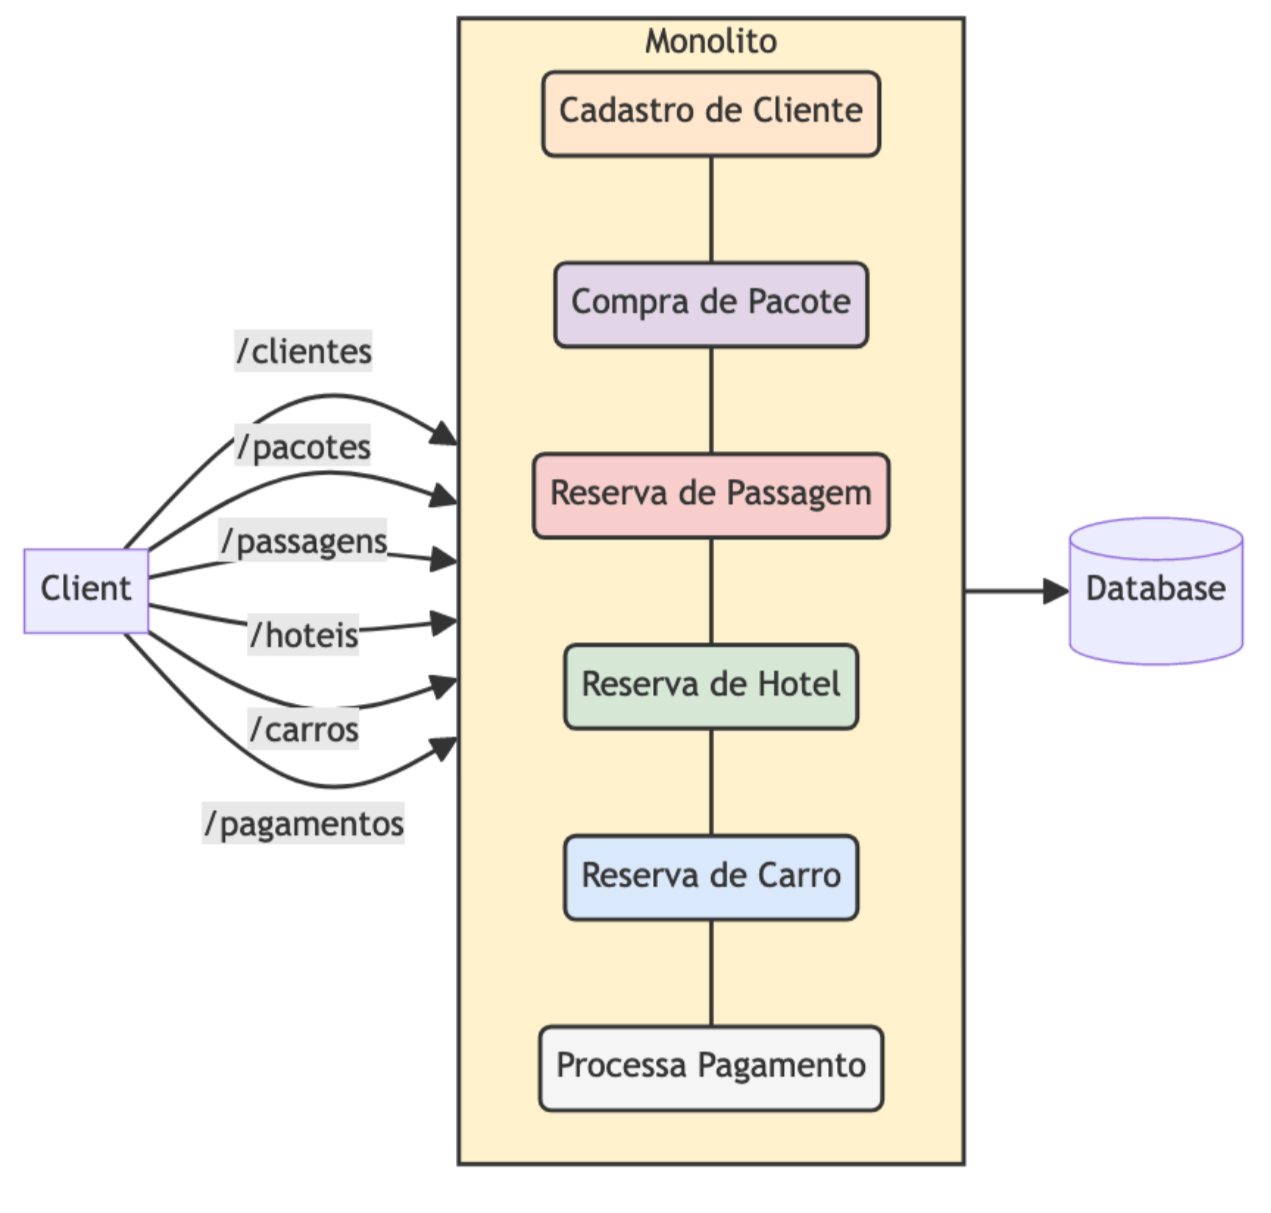
\includegraphics[width=0.8\textwidth]{images/monolito.png}
\caption{Estrutura típica de arquitetura monolítica.}
\label{fig:monolitico}
\end{figure}

Como ilustrado na Figura \ref{fig:monolitico}, o fluxo de requisições percorre camadas internamente acopladas, sem isolamento de processos. Essa centralização explica os resultados empíricos de \cite{farhan2023performance}, onde sistemas monolíticos apresentaram:

\begin{itemize}
\item 40\% maior tempo de resposta sob carga crescente
\item 68\% mais \textit{downtime} durante atualizações
\item Limite máximo de escalonamento em 5 instâncias
\end{itemize}

Limite máximo de escalonamento em 5 instâncias antes de degradação crítica

Apesar das limitações, o modelo mantém relevância em cenários específicos: aplicações com tráfego previsível, equipes co-localizadas, ou quando a simplicidade operacional sobrepõe requisitos de elasticidade \cite{shekhar2023microservices}. Contudo, para sistemas empresariais modernos que demandam entrega contínua e escalabilidade dinâmica, sua viabilidade torna-se progressivamente reduzida.

\subsection{Event-Driven Architecture}
A \textit{Event-Driven Architecture} é especialmente indicada para sistemas que exigem alta escalabilidade e resposta em tempo real. Nesse padrão, os componentes do sistema comunicam-se por meio de eventos, que são processados de forma assíncrona. Essa abordagem é bastante utilizada em sistemas de \textit{e-commerce}, plataformas de \textit{streaming} e aplicações que demandam processamento distribuído, pois permite maior desacoplamento entre os módulos e facilita a escalabilidade horizontal \cite{jamshidi2016systematic}. 

\subsection{Serverless}
Por fim, a arquitetura \textit{serverless} vem ganhando espaço com o avanço das plataformas de computação em nuvem. Nesse modelo, o desenvolvedor se concentra apenas na lógica de negócio, enquanto a infraestrutura é gerenciada automaticamente pelo provedor de nuvem. Isso permite maior agilidade no desenvolvimento e escalabilidade automática, embora traga desafios relacionados à portabilidade e ao controle sobre o ambiente de execução \cite{shekhar2023microservices}.

\begin{figure}[h]
\centering
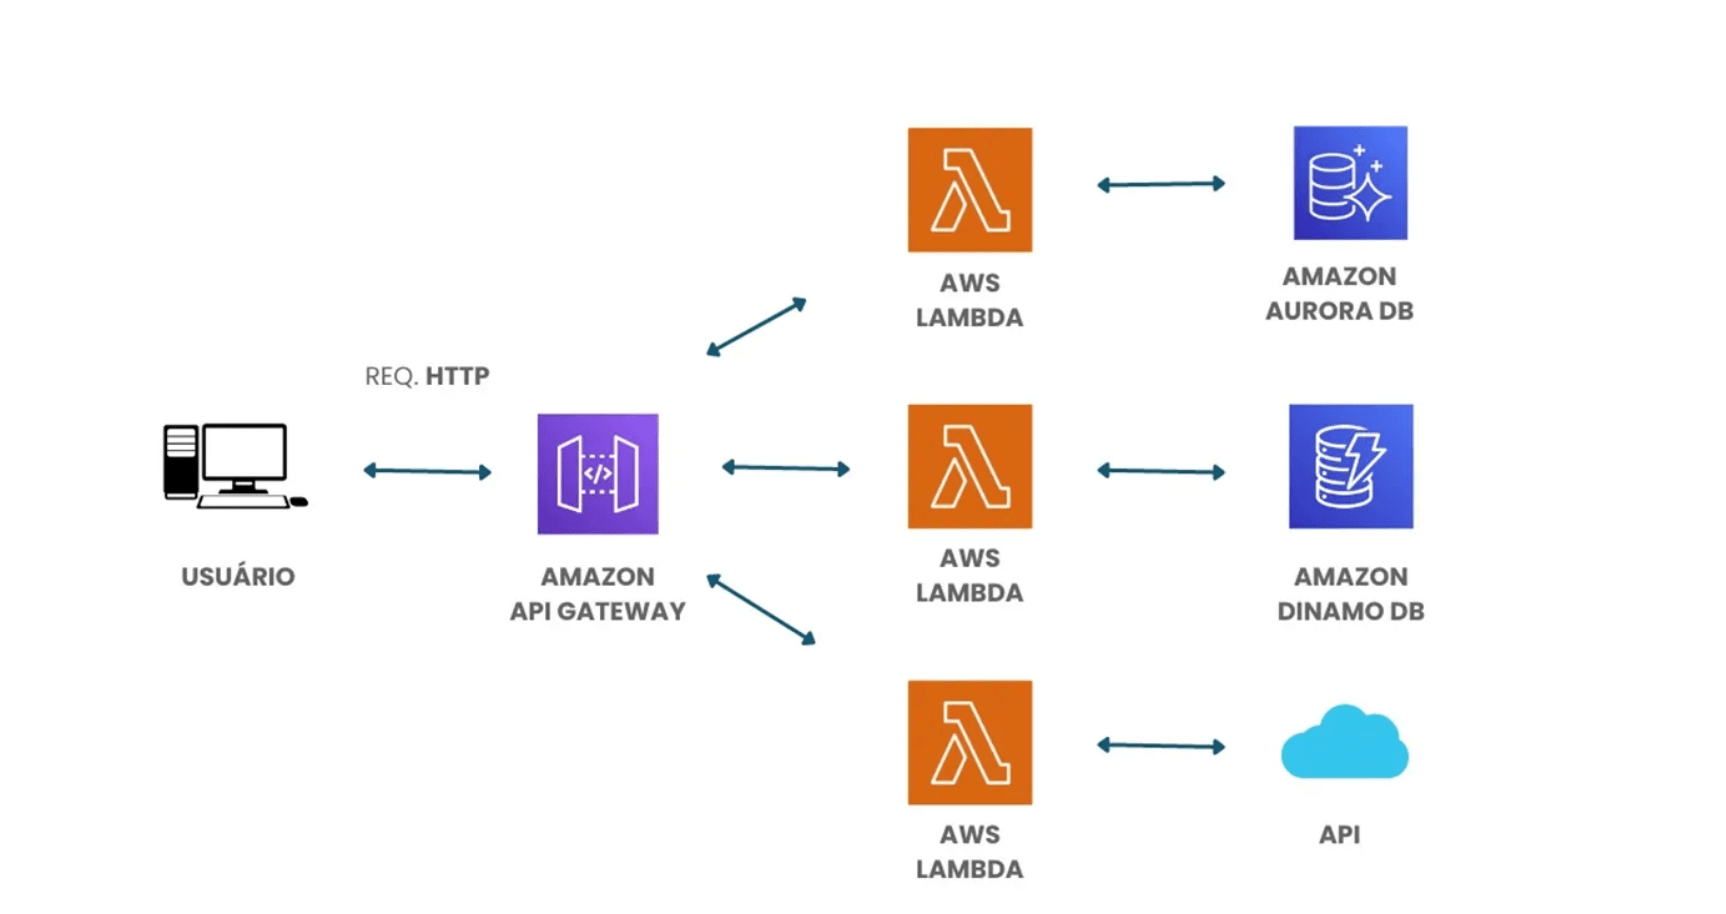
\includegraphics[width=0.9\textwidth]{images/serverless.png}
\caption{Arquitetura Serverless típica, mostrando os componentes principais: API Gateway, Funções como Serviço (FaaS), e serviços gerenciados. Fonte: Adaptado de \cite{shekhar2023microservices}.}
\label{fig:serverless}
\end{figure}

Como ilustrado na Figura \ref{fig:serverless}, a arquitetura serverless consiste em três componentes principais:

\begin{itemize}
    \item \textbf{API Gateway}: Ponto único de entrada para todas as requisições
    \item \textbf{Funções como Serviço (FaaS)}: Execução de código sob demanda (ex: AWS Lambda, Azure Functions)
    \item \textbf{Serviços Gerenciados}: Bancos de dados, filas e armazenamento providos pelo cloud provider
\end{itemize}

Esta abordagem elimina a necessidade de gerenciamento de servidores, permitindo que os desenvolvedores foquem exclusivamente na implementação da lógica de negócios \cite{shekhar2023microservices}.

A escolha do padrão arquitetural mais adequado depende de fatores como requisitos do sistema, contexto de negócio, equipe envolvida e recursos disponíveis. Compreender as vantagens e limitações de cada abordagem é essencial para alinhar a arquitetura às necessidades presentes e futuras do projeto \cite{jamshidi2016systematic, nizami2020comparison}.

\subsection{Microsserviços}
A arquitetura de microsserviços representa uma evolução significativa em relação aos modelos tradicionais de desenvolvimento de software, como a arquitetura monolítica e a \textit{SOA}. Nesse paradigma, o sistema é decomposto em pequenos serviços independentes, cada um responsável por uma funcionalidade específica e comunicando-se por meio de interfaces bem definidas, geralmente via \textit{APIs} \cite{jamshidi2016systematic, nizami2020comparison}. 

Entre os principais benefícios dos microsserviços está a escalabilidade granular, que permite dimensionar apenas os serviços que realmente demandam mais recursos, otimizando custos e desempenho \cite{shekhar2023microservices}. Além disso, a independência entre equipes é favorecida, pois times distintos podem desenvolver, testar e implantar serviços de forma autônoma, acelerando o ciclo de entrega e facilitando a adoção de práticas \textit{DevOps} \cite{nizami2020comparison, farhan2023performance}.

Outro ponto relevante é a resiliência: falhas em um serviço tendem a ser isoladas, reduzindo o impacto sobre o sistema como um todo \cite{farhan2023performance}. Isso é especialmente importante em ambientes de missão crítica, onde a disponibilidade contínua é fundamental. 

No entanto, a adoção de microsserviços também traz desafios consideráveis. A complexidade operacional aumenta, exigindo ferramentas avançadas para orquestração (como \textit{Kubernetes}), monitoramento e observabilidade \cite{jamshidi2016systematic, shekhar2023microservices}. Cada serviço pode demandar sua própria infraestrutura, banco de dados e mecanismos de autenticação, o que eleva a sobrecarga de gerenciamento \cite{nizami2020comparison}.

A observabilidade torna-se um aspecto central, pois a identificação e resolução de falhas em sistemas distribuídos requerem coleta e análise de métricas, \textit{logs} e \textit{traces} distribuídos \cite{observability2023, sha2023automating}. Ferramentas como \textit{Prometheus} e \textit{Jaeger} são amplamente utilizadas para monitorar o desempenho e rastrear requisições entre serviços, facilitando o diagnóstico de problemas e a manutenção da qualidade do sistema \cite{ahmed2022observability}. 

Além disso, a escolha dos protocolos de comunicação entre microsserviços (\textit{\gls{REST}}, \textit{\gls{gRPC}}, \textit{\gls{GraphQL}}) impacta diretamente o desempenho, a flexibilidade e a observabilidade do sistema \cite{niswar2023performance}. Estudos recentes destacam que decisões arquiteturais bem fundamentadas são essenciais para garantir a eficiência e a robustez de sistemas baseados em microsserviços \cite{niswar2023performance, sha2023automating}. 

A arquitetura de microsserviços representa uma evolução paradigmática no desenvolvimento de software, decompondo sistemas complexos em serviços autônomos especializados. Conforme \cite{jamshidi2016systematic}, esta abordagem oferece:

\begin{itemize}
    \item \textbf{Autonomia tecnológica}: Cada serviço pode utilizar linguagens e tecnologias distintas (Java, Python, Node.js)
    \item \textbf{Resiliência aprimorada}: Isolamento de falhas através de padrões como \textit{Circuit Breaker}
    \item \textbf{Entrega contínua}: \textit{Deploys} independentes permitindo múltiplas implantações diárias
\end{itemize}

\subsubsection{Mecanismos de Comunicação}
A comunicação entre serviços ocorre principalmente através de:

\begin{table}[h]
\centering
\caption{Comparação de protocolos de comunicação}
\begin{tabular}{|l|c|c|c|}
\hline
\textbf{Protocolo} & \textbf{Latência} & \textbf{Complexidade} & \textbf{Casos de Uso} \\
\hline
REST/HTTP & Alta & Baixa & Sistemas com baixa frequência \\
gRPC & Baixa & Média & Microserviços acoplados \\
Eventos (Kafka) & Assíncrona & Alta & Sistemas escaláveis \\
\hline
\end{tabular}
\label{tab:protocolos}
\end{table}

Conforme demonstrado na Tabela \ref{tab:protocolos}, a escolha do protocolo impacta diretamente o desempenho do sistema \cite{niswar2023performance}.

\subsubsection{Padrões Arquiteturais Essenciais}
\begin{figure}[h]
\centering
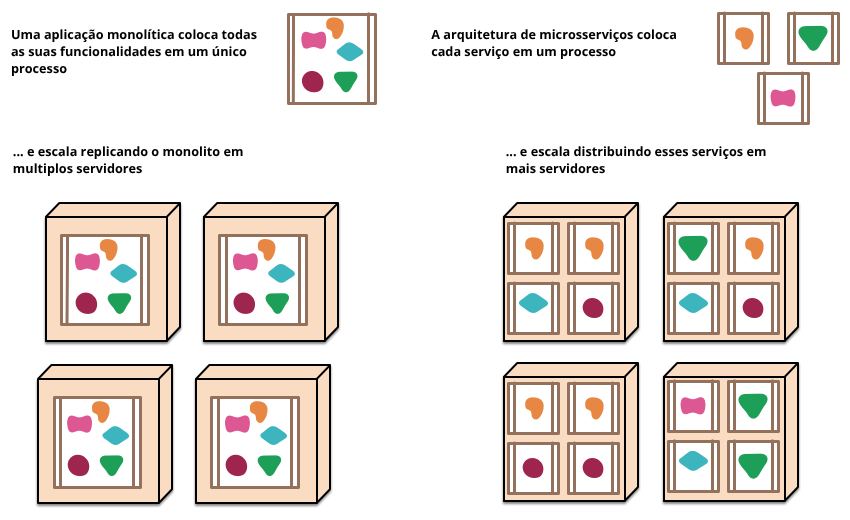
\includegraphics[width=0.85\textwidth]{images/microservice.png}
\caption{Padrões fundamentais em arquitetura de microsserviços}
\label{fig:micro_patterns}
\end{figure}

A Figura \ref{fig:micro_patterns} ilustra as diferenças fundamentais entre a arquitetura monolítica e a arquitetura de microsserviços. À esquerda, observa-se que uma aplicação monolítica agrupa todas as funcionalidades em um único processo. Para escalar esse modelo, é necessário replicar toda a aplicação em múltiplos servidores, o que pode gerar desperdício de recursos e limitações de flexibilidade.

À direita, a arquitetura de microsserviços distribui cada funcionalidade em processos independentes, permitindo que cada serviço seja desenvolvido, implantado e escalado separadamente. Isso proporciona maior eficiência no uso de recursos, facilita a manutenção e possibilita o crescimento gradual do sistema conforme a demanda por funcionalidades específicas.

Essa abordagem modular e distribuída é um dos pilares das arquiteturas modernas voltadas à escalabilidade, resiliência e agilidade no desenvolvimento.

\subsubsection{Desafios Operacionais e Soluções}
A implementação prática enfrenta obstáculos significativos:

\begin{itemize}
    \item \textbf{Observabilidade}: Requer integração de métricas, \textit{logs} e \textit{traces} com ferramentas como:
    \begin{itemize}
        \item \textit{Prometheus} para monitoramento
        \item \textit{Jaeger} para rastreamento distribuído
        \item \textit{EFK Stack} (Elasticsearch, Fluentd, Kibana) para análise
    \end{itemize}
    
    \item \textbf{Orquestração}: Plataformas como \textit{Kubernetes} gerenciam:
    \begin{itemize}
        \item Escalonamento automático
        \item Balanceamento de carga
        \item Recuperação de falhas
    \end{itemize}
\end{itemize}

\subsubsection{Melhores Práticas de Implementação}
Experiências de empresas líderes revelam estratégias eficazes:

\begin{itemize}
    \item \textbf{Amazon}: Utiliza a prática do "time da pizza de dois" — equipes pequenas e independentes, responsáveis por serviços autônomos do início ao fim.
    
    \item \textbf{Netflix}: Introduziu a cultura do \textit{Chaos Engineering}, simulando falhas em produção para garantir a resiliência dos serviços.

    \item \textbf{Spotify}: Estruturou suas equipes em \textit{squads} responsáveis por domínios funcionais, promovendo independência e entrega contínua.

    \item \textbf{Uber}: Implementou uma hierarquia de serviços baseada em criticidade, diferenciando serviços centrais de auxiliares para otimizar a operação.
\end{itemize}

\subsubsection{Casos de Estudo Relevantes}
Resultados empíricos demonstram impactos mensuráveis:

\begin{table}[h]
\centering
\caption{Impacto da migração para microsserviços}
\begin{tabular}{|l|c|c|}
\hline
\textbf{Métrica} & \textbf{Antes} & \textbf{Depois} \\
\hline
Tempo de entrega & 30 dias & 2 dias \\
Disponibilidade & 92\% & 99.95\% \\
Custo de infraestrutura & \$100k/mês & \$65k/mês \\
\hline
\end{tabular}
\label{tab:impacto}
\end{table}

Conforme dados na Tabela \ref{tab:impacto}, organizações reportam melhorias significativas após transição bem-sucedida \cite{farhan2023performance, shekhar2023microservices}.

\subsubsection{Recomendações Estratégicas}
A adoção deve considerar:

\begin{itemize}
    \item \textbf{Pré-requisitos}: Maturidade em DevOps e cultura de automação
    \item \textbf{Critérios}: Complexidade sistêmica > 50k LOC > 15 desenvolvedores
    \item \textbf{Alternativas}: Arquiteturas híbridas para transição gradual
    \item \textbf{Anti-padrões}: Decomposição excessiva ("nanoserviços")
\end{itemize}

Em síntese, microsserviços oferecem vantagens transformacionais para sistemas complexos, mas exigem investimento proporcional em automação e governança \cite{nizami2020comparison, observability2023}.

\subsection{Protocolos de Comunicação para Microsserviços}
A seleção de protocolos de comunicação é um fator crítico em arquiteturas de microsserviços, influenciando diretamente o desempenho, acoplamento e capacidade de evolução do sistema. Dois padrões predominantes neste contexto são \gls{REST} e \gls{gRPC}, cada um com características técnicas distintas que os tornam adequados a cenários específicos \cite{niswar2023performance}.

\subsubsection{\gls{REST} (Representational State Transfer)}
O \gls{REST}, formalizado por Fielding \cite{fielding2000rest} em sua tese seminal, é um estilo arquitetural baseado em princípios de recursos identificáveis por \gls{URI} e operações padronizadas via verbos \gls{HTTP} (GET, POST, PUT, DELETE). Sua adoção generalizada deve-se a:

\begin{itemize}
\item \textbf{Simplicidade}: Uso de formatos legíveis como \gls{JSON}, facilitando depuração e integração entre sistemas heterogêneos. A serialização textual consome 30-50\% mais banda que protocolos binários \cite{niswar2023performance}.
\item \textbf{Estateless}: Cada requisição contém contexto completo, eliminando estado no servidor e favorecendo escalabilidade horizontal \cite{fielding2000rest}.
\item \textbf{Uniform Interface}: Princípios como identificação única de recursos via URI e \gls{HATEOAS} garantem consistência e desacoplamento \cite{maso2024comparativo}.
\item \textbf{Compatibilidade}: Suporte nativo em navegadores e adoção massiva em APIs públicas \cite{maso2024comparativo}.
\end{itemize}

\textbf{Limitações em cenários complexos}:
\begin{itemize}
\item \textbf{Overhead de comunicação}: Serialização textual aumenta latência e consumo de \gls{CPU}, especialmente em payloads grandes \cite{niswar2023performance}.
\item \textbf{Modelo síncrono}: Suporta apenas comunicação unária (request/response), inviabilizando fluxos assíncronos \cite{niswar2023performance}.
\item \textbf{Falta de contratos rígidos}: Validação de esquemas depende de implementações adicionais \cite{maso2024comparativo}.
\end{itemize}

\textbf{Operações Básicas e Códigos HTTP}:
A Tabela \ref{tab:rest_operations} sintetiza o mapeamento CRUD em REST, conforme padrões industriais \cite{fielding2000rest}:

\begin{table}[h]
\centering
\caption{Operações REST e códigos HTTP}
\label{tab:rest_operations}
\begin{tabular}{|l|c|c|}
\hline
\textbf{Método HTTP} & \textbf{Ação} & \textbf{Código Sucesso} \\ \hline
GET & Ler recurso & 200 (OK) \\ \hline
POST & Criar recurso & 201 (Created) \\ \hline
PUT/PATCH & Atualizar recurso & 200 (OK) ou 204 (No Content) \\ \hline
DELETE & Excluir recurso & 204 (No Content) \\ \hline
\end{tabular}
\fonte{Adaptado de \cite{niswar2023performance} e \cite{fielding2000rest}.}
\end{table}

% \begin{figure}[h]
% \centering
% \includegraphics[width=0.75\textwidth]{images/rest-protocol.png}
% \caption{Fluxo de comunicação REST típico com operações CRUD sobre recursos. Fonte: Adaptado de \cite{aws:1}.}
% \label{fig:rest_flow}
% \end{figure}

\subsubsection{\gls{gRPC} (gRPC Remote Procedure Calls)}
Desenvolvido pelo Google e inicialmente lançado em 2015 \cite{googleblog:5}, o \gls{gRPC} é um \textit{framework} aberto de alta performance para chamadas de procedimento remoto (RPC) que utiliza \gls{HTTP/2} e \textit{Protocol Buffers} para comunicação binária eficiente. Conforme demonstrado por \cite{niswar2023performance}, sua adoção em arquiteturas de microsserviços deve-se aos seguintes diferenciais:

\begin{itemize}
\item \textbf{Desempenho superior}: A serialização binária via \textit{Protocol Buffers} reduz o tamanho dos \textit{payloads} em até 80\% e a latência em 60\% comparado a APIs REST tradicionais, conforme mensurações em ambientes controlados \cite{niswar2023performance}.
\item \textbf{Streaming bidirecional}: Suporte nativo a fluxos contínuos de dados (cliente-servidor, servidor-cliente e bidirecional), habilitando comunicação assíncrona para aplicações em tempo real \cite{grpc:1}.
\item \textbf{Contratos fortemente tipados}: Definição explícita de serviços e estruturas de mensagens em arquivos \texttt{.proto}, garantindo compatibilidade e evolução controlada de APIs \cite{maso2024comparativo}.
\item \textbf{Geração de código automática}: Compilação de \textit{stubs} clientes e servidores em 11 linguagens de programação a partir de arquivos \texttt{.proto}, promovendo consistência e redução de erros \cite{grpc:1}.
\end{itemize}

\textbf{Aspectos críticos em sua adoção}:
\begin{itemize}
\item \textbf{Acoplamento forte}: Alterações nos contratos \texttt{.proto} exigem atualização sincronizada de clientes e servidores, aumentando a complexidade de evolução em sistemas distribuídos \cite{ibm:7}.
\item \textbf{Suporte limitado em navegadores}: A ausência de implementação nativa do HTTP/2 em navegadores requer o uso do proxy \textit{gRPC-Web} para comunicações cliente-web \cite{wallarm:4}.
\item \textbf{Curva de aprendizagem}: Complexidade na definição de contratos e manipulação de fluxos de \textit{streaming}, especialmente para desenvolvedores familiarizados com paradigmas REST \cite{marutitech:9}.
\end{itemize}

\textbf{Modelos de Comunicação}:
A Figura \ref{fig:grpc_streaming} ilustra os quatro padrões suportados:

\begin{figure}[h]
\centering
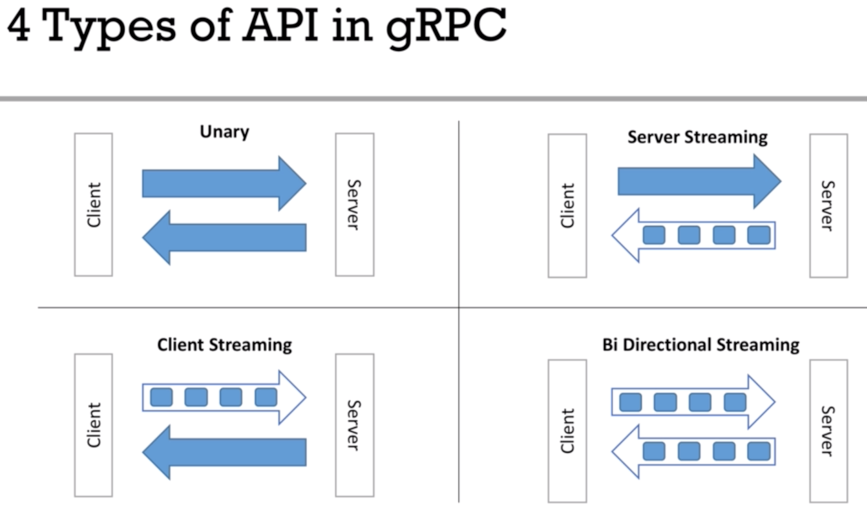
\includegraphics[width=0.9\textwidth]{images/grpc.png}
\caption{Padrões de streaming no gRPC: (A) Unário, (B) Servidor, (C) Cliente, (D) Bidirecional.}
\label{fig:grpc_streaming}
\end{figure}

\textbf{Vantagens Técnicas Comprovadas}:
Estudos empíricos demonstram ganhos operacionais mensuráveis \cite{niswar2023performance}:
\begin{itemize}
\item Redução de 35-45\% no consumo de CPU durante serialização
\item Até 7x maior throughput em comunicações inter-serviços
\end{itemize}

% \ref{cap:Introducao}).
% \ref{cap:Introducao}).
% % ----------------------------------------------------------
% \section{CONCEITOS EXPLORADOS NO TRABALHO}\label{sec:conceitos}
% % ----------------------------------------------------------

% Para cada conceito explorado no trabalho, você deve criar nova uma seção como esta, por exemplo: “2.1 INTERNET DAS COISAS”.

% % ----------------------------------------------------------
% \section{TECNOLOGIAS UTILIZADAS NO DESENVOLVIMENTO}\label{sec:tecnologias}
% % ----------------------------------------------------------

% Para cada tecnologia utilizada no desenvolvimento, você deve criar uma nova seção como esta, por exemplo: “2.2 PLATAFORMA ARDUINO”.

% ----------------------------------------------------------
% \section{Exemplo citação longa em Látex} \label{}
% ----------------------------------------------------------


% \begin{citacao}
% 	Após a ilustração, na parte inferior, indicar a fonte consultada (elemento obrigatório, mesmo que seja produção do próprio autor), legenda, notas e outras informações necessárias à sua compreensão (se houver). A ilustração deve ser citada no texto e inserida o mais próximo possível do texto a que se refere. \cite[p. 11]{gil2008metodos}.
% \end{citacao}

% % ----------------------------------------------------------
% \section{Exemplo Equações e fórmulas em Látex}
% % ----------------------------------------------------------

% As equações e fórmulas devem ser destacadas no texto para facilitar a leitura. Para numerá-las, usar algarismos arábicos entre parênteses e alinhados à direita. Pode-se adotar uma entrelinha maior do que a usada no texto.

% Exemplos, \ref{eq:Eq_1} e \ref{eq:Eq_2}.

% \begin{equation}\label{eq:Eq_1}
% C = 2 \pi r
% \end{equation}

% \begin{equation}\label{eq:Eq_2}
% \gls{A} = \gls{pi} \gls{r}^2
% \end{equation}


% % ----------------------------------------------------------
% \section{Exemplo Código-Fonte}
% % ----------------------------------------------------------

% Os trechos de código devem ser exibidos em formatação de código com linhas enumeradas sequenciais a esquerda para falicitar os comentários. Abaixo segue exemplos carregando o código através de um arquivo e digitando diretamente no texto.

% \lstinputlisting[
%     language=C, % Defina a linguagem do código
%     numbers=left, % Exibir números de linha à esquerda
%     %linerange={23-66}, % Defina os intervalos de linhas
%     firstnumber={1}, % Números iniciais correspondentes aos intervalos
%     stepnumber=1, % Incremento do número de linha
%     caption={Exemplo carregando arquivo...},
%     label=src:sample_c
% ]{sources/sample.c}

% \begin{lstlisting}[language=json, caption={Exemplo de Dados JSON}, label={src:json}]
%     {
%         "name": "John Doe",
%         "age": 30,
%         "address": {
%             "street": "1234 Main St",
%             "city": "Anytown",
%             "state": "CA",
%             "zip": "12345"
%         },
%         "phoneNumbers": [
%             {"type": "home", "number": "555-1234"},
%             {"type": "work", "number": "555-5678"}
%         ]
%     }
%     \end{lstlisting}


% \begin{lstlisting}[language=C, caption={Exemplo digitado no texto}, label={src:codigo_2}]
% 	#include <stdio.h>
	
% 	void main(){
% 		printf("Olá Mundo!");
% 	}
% 	\end{lstlisting}

% Exemplos, \ref{src:sample_c}, \ref{src:json} e \ref{src:codigo_2}.

